\documentclass[12pt,a4paper]{article}
\usepackage{amsmath}
\usepackage{graphicx}
\usepackage{geometry}
\usepackage{float}
\geometry{left=2cm,right=2cm,top=2.5cm,bottom=2.5cm}

\title{\textbf{Branch 2 (Degenerated 4-Bar) Analysis Report \\ with Explicit Matrix Operations}}
\author{Automated Generation System}
\date{\today}

\begin{document}
\maketitle

\section{Mathematical Formulation}
For this specific branch, the topological constraint locks joints $J_2, J_4,$ and $J_6$ to zero. The driving joint is $J_3$. The full kinematic constraint $T_1 \dots T_7 = I$ is reduced to three active variables ($q_1, q_5, q_7$).
The velocity constraint yields $J_p \dot{\mathbf{q}}_p = - J_a \dot{q}_3$, where $J_p \in \mathbb{R}^{6 \times 6}$ is the passive Jacobian matrix obtained by removing the column corresponding to the driving joint $J_3$.

\section{Example Matrix Calculation at $q_3 = 0^\circ$}
The solved full joint configuration (in radians), showing the locked joints explicitly as $0$, is:
\begin{equation}
    \mathbf{q} = \begin{bmatrix} -0.0000 \\ 0.0000 \\ 0.0000 \\ 0.0000 \\ -0.0000 \\ 0.0000 \\ 0.0000 \end{bmatrix}
\end{equation}

Based on this configuration, the full $6 \times 7$ Jacobian matrix $J$ is evaluated as:
\begin{equation}
    \resizebox{0.95\textwidth}{!}{$ J = \begin{bmatrix}
  -0.000 & -0.000 & -0.000 & 2.500 & -0.000 & -2.500 & 0.000 \\
  0.000 & -1.000 & -0.000 & 3.000 & -0.000 & 2.000 & 0.000 \\
  0.000 & 0.000 & -3.000 & -0.000 & -0.500 & 0.000 & -2.000 \\
  0.000 & 0.000 & -0.000 & -0.000 & -0.000 & 0.000 & 0.000 \\
  0.000 & 0.000 & -1.000 & -0.000 & -1.000 & 0.000 & 1.000 \\
  1.000 & 1.000 & 0.000 & -1.000 & 0.000 & 1.000 & 0.000
\end{bmatrix} $}
\end{equation}

Extracting the columns of the passive joints yields $J_p \in \mathbb{R}^{6 \times 6}$:
\begin{equation}
    \resizebox{0.85\textwidth}{!}{$ J_p = \begin{bmatrix}
  -0.000 & -0.000 & 2.500 & -0.000 & -2.500 & 0.000 \\
  0.000 & -1.000 & 3.000 & -0.000 & 2.000 & 0.000 \\
  0.000 & 0.000 & -0.000 & -0.500 & 0.000 & -2.000 \\
  0.000 & 0.000 & -0.000 & -0.000 & 0.000 & 0.000 \\
  0.000 & 0.000 & -0.000 & -1.000 & 0.000 & 1.000 \\
  1.000 & 1.000 & -1.000 & 0.000 & 1.000 & 0.000
\end{bmatrix} $}
\end{equation}

Applying Singular Value Decomposition (SVD) on $J_p = U \Sigma V^T$:
\begin{equation}
    \resizebox{0.85\textwidth}{!}{$ U = \begin{bmatrix}
  -0.667 & 0.626 & -0.000 & -0.405 & 0.000 & 0.000 \\
  -0.662 & -0.747 & 0.000 & -0.066 & -0.000 & -0.000 \\
  0.000 & 0.000 & 0.894 & 0.000 & -0.447 & -0.000 \\
  -0.000 & -0.000 & -0.000 & -0.000 & -0.000 & -1.000 \\
  -0.000 & -0.000 & -0.447 & -0.000 & -0.894 & 0.000 \\
  0.343 & -0.224 & 0.000 & -0.912 & 0.000 & 0.000
\end{bmatrix} $}
\end{equation}
\begin{equation}
    \resizebox{0.85\textwidth}{!}{$ \Sigma = \begin{bmatrix}
  4.190 & 0.000 & 0.000 & 0.000 & 0.000 & 0.000 \\
  0.000 & 3.362 & 0.000 & 0.000 & 0.000 & 0.000 \\
  0.000 & 0.000 & 2.236 & 0.000 & 0.000 & 0.000 \\
  0.000 & 0.000 & 0.000 & 1.280 & 0.000 & 0.000 \\
  0.000 & 0.000 & 0.000 & 0.000 & 1.118 & 0.000 \\
  0.000 & 0.000 & 0.000 & 0.000 & 0.000 & 0.000
\end{bmatrix} $}
\end{equation}
\begin{equation}
    \resizebox{0.85\textwidth}{!}{$ V^T = \begin{bmatrix}
  0.082 & 0.240 & -0.953 & 0.000 & 0.164 & -0.000 \\
  -0.067 & 0.156 & -0.134 & -0.000 & -0.976 & -0.000 \\
  0.000 & -0.000 & 0.000 & 0.000 & 0.000 & -1.000 \\
  -0.713 & -0.661 & -0.232 & 0.000 & -0.025 & -0.000 \\
  0.000 & 0.000 & 0.000 & 1.000 & -0.000 & 0.000 \\
  0.693 & -0.693 & -0.139 & 0.000 & -0.139 & 0.000
\end{bmatrix} $}
\end{equation}

\section{Analysis Results \& Curve Fitting}
\begin{figure}[H]
    \centering
    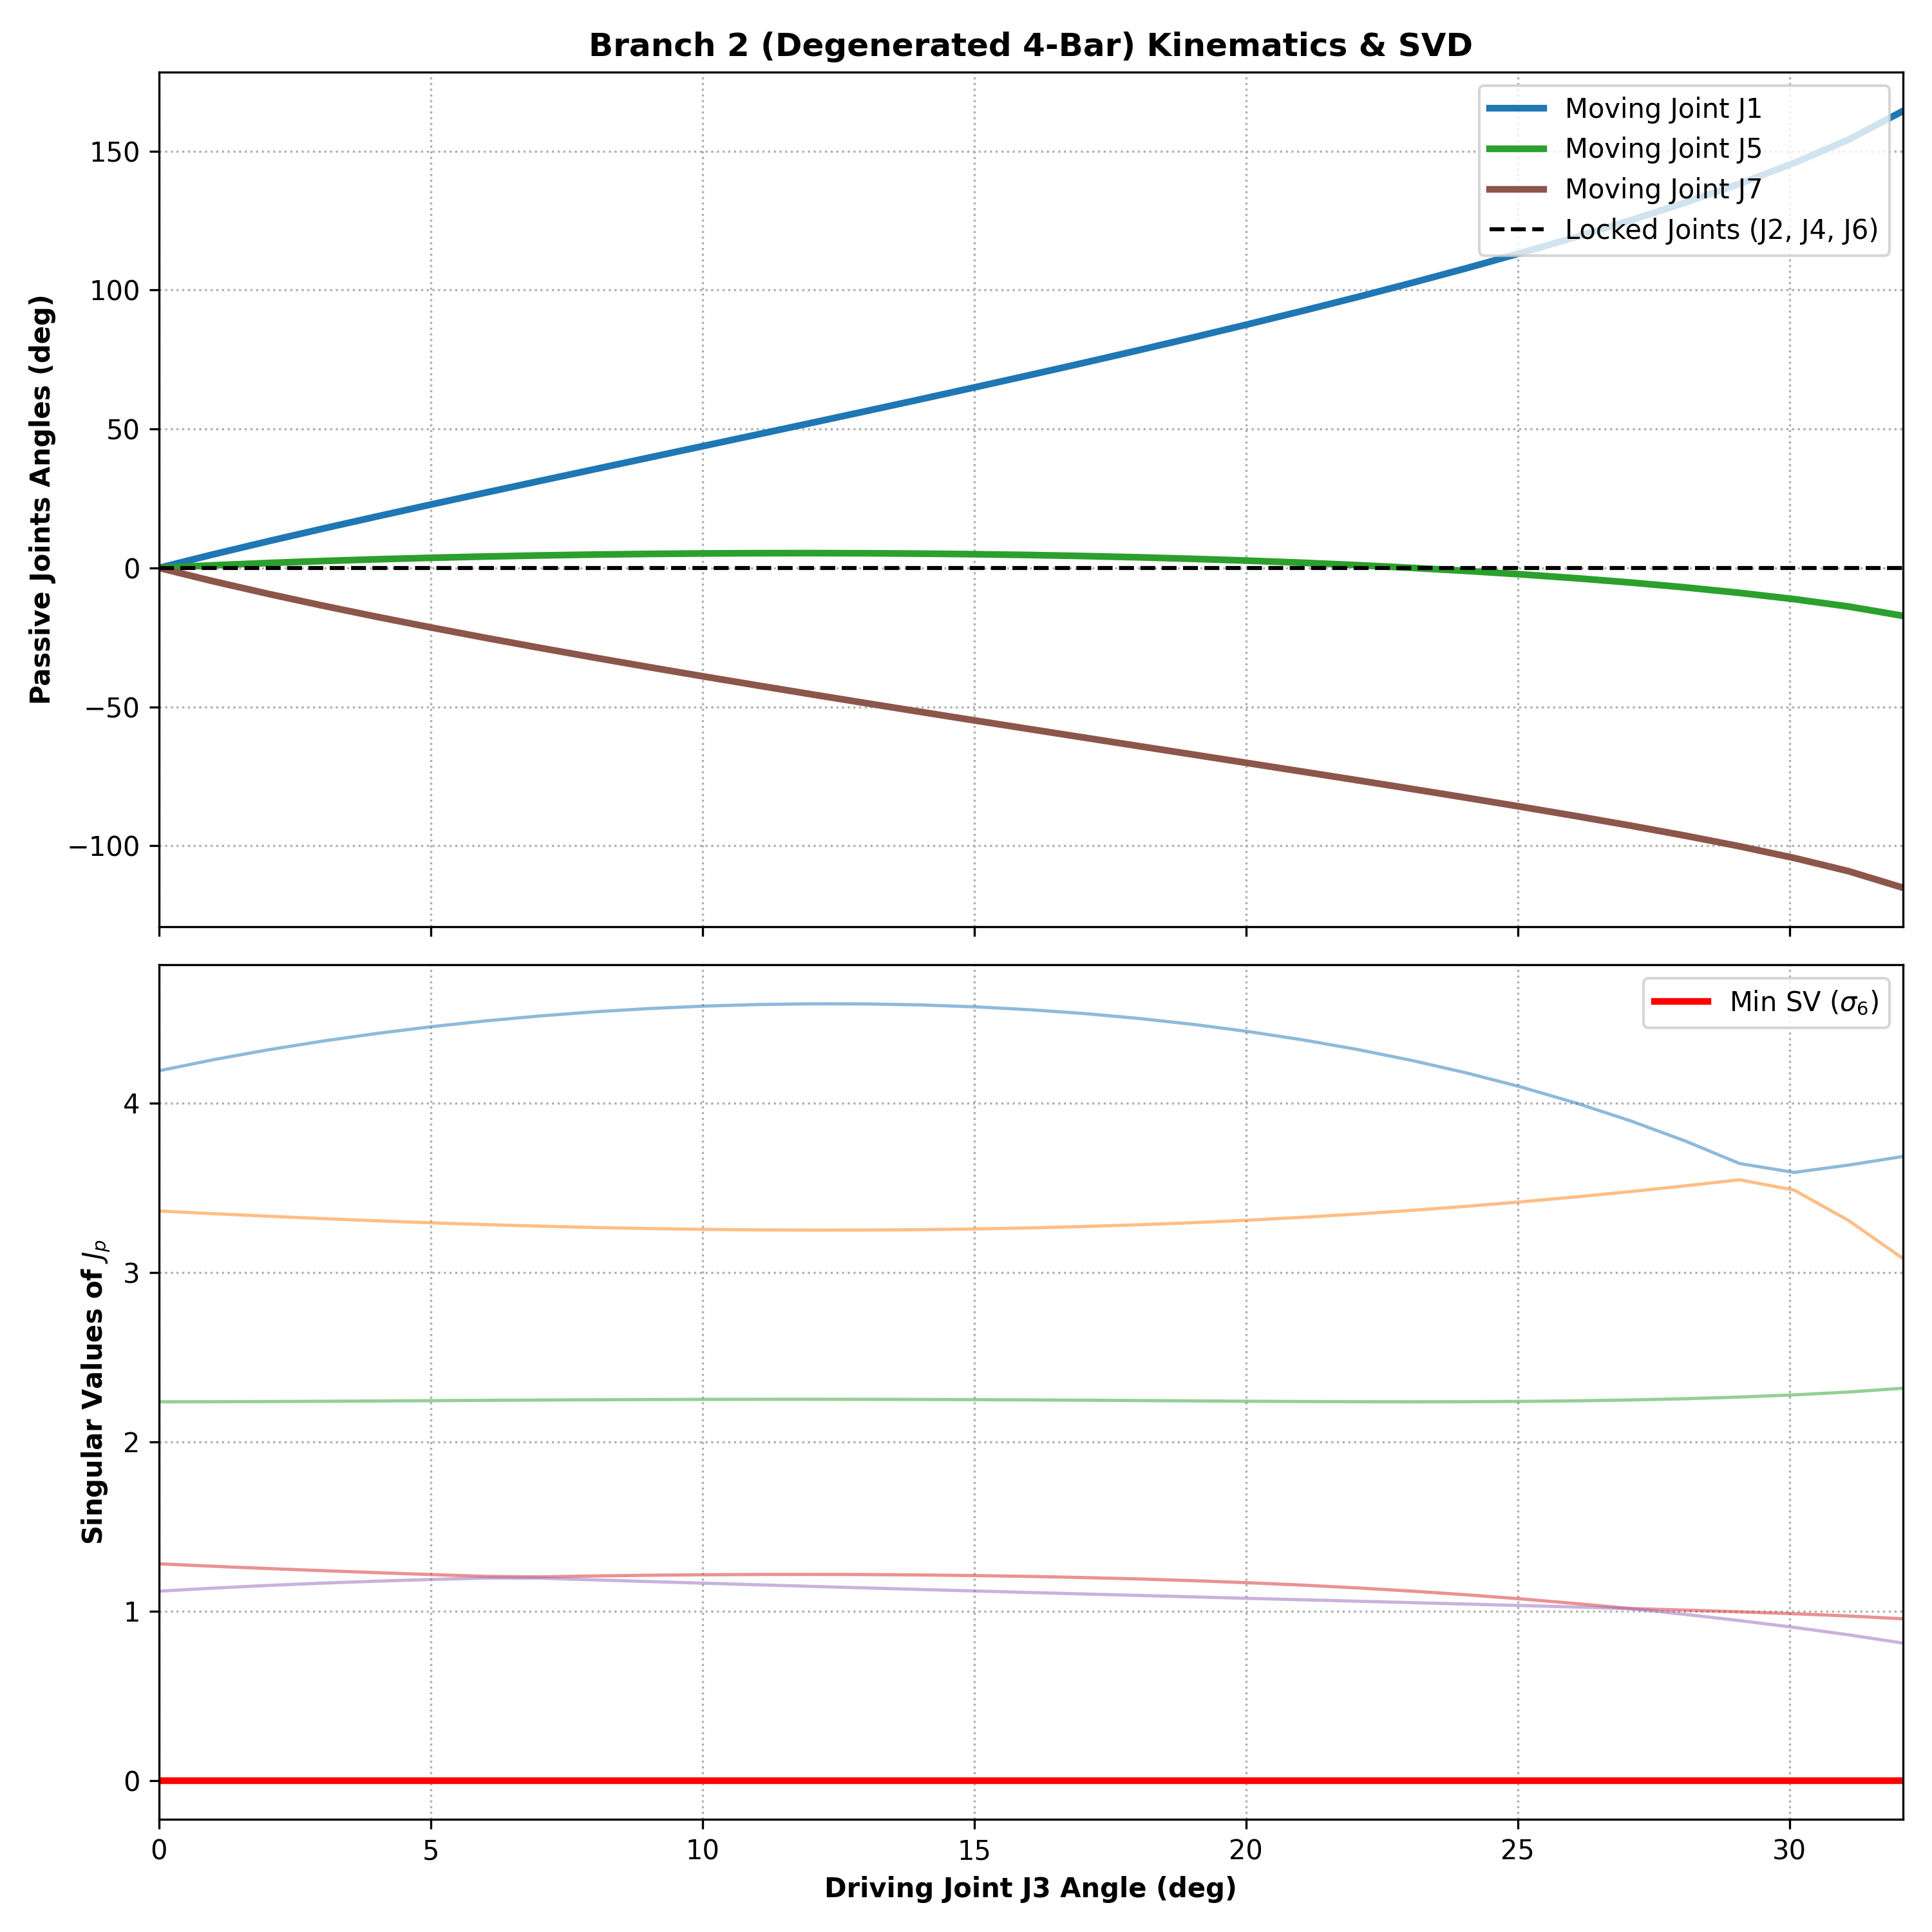
\includegraphics[width=0.9\textwidth]{branch2_q3_analysis.png}
    \caption{Kinematic mapping and singular value evolution driven by $J_3$ on Branch 2.}
\end{figure}

The Fourier series expressions for the \textbf{moving} passive joints are:
\begin{itemize}
\item \textbf{Joint J1:} \\ $Q_{J1}(x) = +295246.095 -433177.915\cos(x) -97759.163\sin(x) +161643.091\cos(2x) +77370.455\sin(2x) -23711.147\cos(3x) -18904.486\sin(3x)$
\item \textbf{Joint J5:} \\ $Q_{J5}(x) = -115151.694 +167713.559\cos(x) +41668.084\sin(x) -61192.262\cos(2x) -32466.924\sin(2x) +8630.367\cos(3x) +7775.662\sin(3x)$
\item \textbf{Joint J7:} \\ $Q_{J7}(x) = -179423.214 +264492.669\cos(x) +55900.899\sin(x) -100103.702\cos(2x) -44706.010\sin(2x) +15034.155\cos(3x) +11079.610\sin(3x)$
\end{itemize}
\end{document}
